%%%%%%%%%%%%%%%%%%%%%%%%%%%%%%%%%%%%%%%%%%%%%%%%%%%%%%%%%%%%%%%%%%%%%%%%%%%%%
%% Original default rstudio/pandoc latex file
%% upated by @jhollist 09/15/2014
%% inspired by @cboetting https://github.com/cboettig/template and
%% @rmflight blog posts:
%% http://rmflight.github.io/posts/2014/07/analyses_as_packages.html 
%% http://rmflight.github.io/posts/2014/07/vignetteAnalysis.html).  
%%%%%%%%%%%%%%%%%%%%%%%%%%%%%%%%%%%%%%%%%%%%%%%%%%%%%%%%%%%%%%%%%%%%%%%%%%%%%

\documentclass[11pt,a4paper]{article}
\usepackage[T1]{fontenc}
\usepackage{lmodern}
\usepackage{amssymb,amsmath}
\usepackage{ifxetex,ifluatex}
\usepackage{fixltx2e} % provides \textsubscript
% use upquote if available, for straight quotes in verbatim environments
\IfFileExists{upquote.sty}{\usepackage{upquote}}{}
\ifnum 0\ifxetex 1\fi\ifluatex 1\fi=0 % if pdftex
  \usepackage[utf8]{inputenc}
\else % if luatex or xelatex
  \ifxetex
    \usepackage{mathspec}
    \usepackage{xltxtra,xunicode}
  \else
    \usepackage{fontspec}
  \fi
  \defaultfontfeatures{Mapping=tex-text,Scale=MatchLowercase}
  \newcommand{\euro}{€}
\fi
% use microtype if available
\IfFileExists{microtype.sty}{\usepackage{microtype}}{}
\usepackage[margin=1in]{geometry}
\usepackage{longtable,booktabs}
\usepackage{graphicx}
% Redefine \includegraphics so that, unless explicit options are
% given, the image width will not exceed the width of the page.
% Images get their normal width if they fit onto the page, but
% are scaled down if they would overflow the margins.
\makeatletter
\def\ScaleIfNeeded{%
  \ifdim\Gin@nat@width>\linewidth
    \linewidth
  \else
    \Gin@nat@width
  \fi
}
\makeatother
\let\Oldincludegraphics\includegraphics
{%
 \catcode`\@=11\relax%
 \gdef\includegraphics{\@ifnextchar[{\Oldincludegraphics}{\Oldincludegraphics[width=\ScaleIfNeeded]}}%
}%
\ifxetex
  \usepackage[setpagesize=false, % page size defined by xetex
              unicode=false, % unicode breaks when used with xetex
              xetex]{hyperref}
\else
  \usepackage[unicode=true]{hyperref}
\fi
\hypersetup{breaklinks=true,
            bookmarks=true,
            pdfauthor={},
            pdftitle={working title Compatibility system and stigma size are the main predictors of heterospecific pollen effect},
            colorlinks=true,
            citecolor=blue,
            urlcolor=blue,
            linkcolor=magenta,
            pdfborder={0 0 0}}
\urlstyle{same}  % don't use monospace font for urls
\setlength{\parindent}{0pt}
\setlength{\parskip}{6pt plus 2pt minus 1pt}
\setlength{\emergencystretch}{3em}  % prevent overfull lines
\setcounter{secnumdepth}{0}

%%%%%%%%%%%%%%%%%%%%%%%%%%%%%%%%%%%%%%%%%%%%%%%%%%%%%%%%
%Changes borrowed from @cboettig, added by @jhollist 
% A modified page layout 
\textwidth 6.75in
\oddsidemargin -0.15in
\evensidemargin -0.15in
\textheight 9in
\topmargin -0.5in
\usepackage{lineno} % add 
  \linenumbers % turns line numbering on 
%%%%%%%%%%%%%%%%%%%%%%%%%%%%%%%%%%%%%%%%%%%%%%%%%%%%%%%%

%%%%%%%%%%%%%%%%%%%%%%%%%%%%%%%%%%%%%%%%%%%%%%%%%%%%%%%%
%%Packages and layout changes by @jhollist 09/15/2014
\usepackage{ragged2e}
\usepackage[font=normalsize]{caption}
  \usepackage[doublespacing]{setspace}
\usepackage{parskip}
\usepackage{fancyhdr}
\pagestyle{fancy}
\fancyhf{}
\renewcommand{\headrulewidth}{0pt}
  \rfoot{\today}
\lfoot{\thepage}
%%Changed default abstract width and added lines
\renewenvironment{abstract}{
  \hfill\begin{minipage}{1\textwidth}
  \rule{\textwidth}{1pt}\vspace{5pt}
  \normalsize
  \begin{justify}
  \bfseries\abstractname\vspace{5pt}
  \end{justify}}
  {\par\noindent\rule{\textwidth}{1pt}\end{minipage}
}
%%%%%%%%%%%%%%%%%%%%%%%%%%%%%%%%%%%%%%%%%%%%%%%%%%%%%%%%

\title{working title Compatibility system and stigma size are the main
predictors of heterospecific pollen effect}
\author{
Jose B. Lanuza
Ignasi Bartomeus
Tia-Lynn Ashman
Romina Rader
}
\date{}
% Allowing for landscape pages
\usepackage{lscape}
\newcommand{\blandscape}{\begin{landscape}}
\newcommand{\elandscape}{\end{landscape}}

% Left justification of the text: see https://www.sharelatex.com/learn/Text_alignment
% \usepackage[document]{ragged2e} % already in the latex template
\newcommand{\bleft}{\begin{flushleft}}
\newcommand{\eleft}{\end{flushleft}}

%%Fix tightlist error: https://stackoverflow.com/questions/40438037/tightlist-error-using-pandoc-with-markdown
%%Added 2018-03-26 
\providecommand{\tightlist}{%
  \setlength{\itemsep}{0pt}\setlength{\parskip}{0pt}}
%%%  
  

\begin{document}
%%Edited by @jhollist 09/15/2014
%%Adds title from YAML
\begin{singlespace}
\begin{center}
\huge working title Compatibility system and stigma size are the main
predictors of heterospecific pollen effect
\end{center}
%%Adds Author, correspond email asterisk, and affilnum from YAML
\begin{center}
\large
Jose B. Lanuza \textsuperscript{*} \textsuperscript{1} 
Ignasi Bartomeus \textsuperscript{2} 
Tia-Lynn Ashman \textsuperscript{3} 
Romina Rader \textsuperscript{1} 
\end{center}
%%Adds affiliations from YAML
\begin{justify}
\footnotesize \emph{ 
\\*
\textsuperscript{1}University of New England (Australia)\\*
\\*
\textsuperscript{2}Estacion Biologica de Donana (EBD-CSIC), E-41092 Sevilla, Spain\\*
\\*
\textsuperscript{3}Department of Biological Sciences, University of Pittsburgh 4249 Fifth
Avenue, Pittsburgh, Pennsylvania 15260-3929 USA\\*
}
%%Adds corresponding author email(s) from YAML
\newcounter{num}
\setcounter{num}{1}
\\[0.1cm]
\footnotesize \emph{ 
\ifnum\value{num}=1%
\textsuperscript{*} corresponding author:
\fi
\href{mailto:barragansljose@gmail.com}{\nolinkurl{barragansljose@gmail.com}}
\stepcounter{num}
}
\end{justify}
%%Adds date from YAML
\normalsize

\end{singlespace}


\singlespace

\vspace{2mm}\hrule

Pollinator sharing can have negative consequences for plant fitness with
the arrival of foreign pollen. However, the costs of heterospecific
pollen are not yet well understood. We conducted a glasshouse experiment
to understand how phylogenetic relatedness and plant traits mediate the
impacts of heterospecific pollen transfer. We conducted 1800 crosses by
experimentally transferring pollen (50\% and 100\% ratio) with
reciprocal crosses between 10 species belonging to three different
families: Brassicaceae, Solanaceae and Convolvulaceae. Seed set was used
as proxy of plant fitness. We found that for 65\% of the treatments with
50\% mix reduced seed set. Moreover, the reduction in seed set was
dependent on the degree of relatedness and reproductive traits of the
pollen recipient and not the pollen donor. Our results show that certain
traits, particularly compatibility system, are critical in understanding
the costs of heterospecific pollen. \vspace{3mm}\hrule

\emph{Keywords}: heterospecific pollen, plant reproduction, fitness,
interspecific competition, phylogenetic distance.

\doublespace

\bleft

\section{INTRODUCTION}\label{introduction}

In most ecosystems, plant species normally coexist and share their
floral visitors with other species Waser et al. (1996). From the plants'
perspective, pollinator sharing can be positive for some plants
Carvalheiro et al. (2014) or negative for others Pauw (2013), depending
on the facilitation gradient. An increasing number of visits often
correlates with higher chances of fertilization Engel and Irwin (2003).
However this is not always the case, among these possible flower
visitors there are also nectar robbers and pollen thieves Inouye (1980);
Magrach et al. (2017). Receiving both sufficient quantity and quality
deposited on the stigma is thus highly relevant to the pollination
success of the plant Aizen and Harder (2007).

By visiting many plant species, many pollinators are responsible for
conspecific pollen loss and the transport of foreign pollen, both of
which can have important detrimental effects on species fitness Morales
and Traveset (2008); Ashman and Arceo-Gómez (2013); Arceo-Gómez and
Ashman (2016). Foreign pollen arrival can play an important role in
plant species fitness but outcomes are variable and appear to be context
dependent as there is not always a decrease in fitness Morales and
Traveset (2008). Some of this variation is likely due to the enormous
variability of foreign pollen transferred across systems ranging from 0
to 75 percent. However, most studies report ranges of heterospecific
pollen between 0 and 20 percent of the total pollen load Bartomeus et
al. (2008) Montgomery and Rathcke (2012); Ashman and Arceo-Gómez (2013);
Fang and Huang (2013), yet even these relatively low amounts of
heterospecific pollen transferred can decrease fitness greatly Thomson
et al. (1982). While we now have some understanding of the impacts of
heterospecific pollen quantity, we have less understanding of other
factors that could be driving the variation in impacts upon fitness.
Ashman and Arceo-Gómez (2013) postulated the first predictive framework
that identifies a need to understand how plant traits might mediate
heterospecific pollen effect, whereby mating system and pollen size were
predicted to potentially mediate the impact of foreign pollen transfer
on plant fitness. This concept is supported by specific case studies,
such as Tong and Huang (2016) that demonstrate an asymmetrical effect in
6 species of \emph{Pedicularis} whereby the pollen of long styled
species was able to grow the full length of the style on short styled
species but not vice versa. While this suggests that the impacts of
heterospecific pollen may differ among pollen donor and recipient, few
studies have been conducted to ascertain whether this pattern is in fact
a general trend or to identify the extent to which other plant traits
are critical to heterospecific pollen impacts.

Plant traits are crucial to understand heterospecific pollen effect but
the multifactorial nature of the traits that are involve in the
pollen-pistil interaction make difficult to unravel what are the main
traits in driving the effect. These traits can be seen from a male
perspective of both donor and recipient where pollen size, pollen
aperture number and pollen allelopathy are key components to understand
the outcome of foreign pollen arrival Murphy and Aarssen (1995); Ashman
and Arceo-Gómez (2013). In Ashman and Arceo-Gómez (2013) small pollen is
predicted to cause a greater fitness decrease, although this can be true
there are also other possibilities to consider which can obscure a
predictive framework like big pollen can clogg small stigmas with fewer
pollen grains, bigger stigmas are less likely to be clogged by small
pollen grains and bigger pollen can outcompete smaller pollen grains due
to faster pollen tube growth rate Williams and Rouse (1990). Moreover,
to understand the different mechanical or chemical effects of pollen
also the female traits of the pollen recipient have to be considered,
from the literature these main traits are: stigma size, style length,
number of ovules, incompatibility system and also a structural trait
such as flower morphology Montgomery and Rathcke (2012); Ashman and
Arceo-Gómez (2013); Tong and Huang (2016). For example, greater
stigmatic area is positively correlated with greater heterospecific
pollen deposition Montgomery and Rathcke (2012) and therefore possibly
with an increase in negative effect. For species that are
self-incompatible the barriers towards heterospecific pollen are
stronger than self-compatible species Ashman and Arceo-Gómez (2013).
Nonetheless, an effect of foreign pollen is a bit obscured by the
variability within species, however species that are strong selfers or
strong outcrossers have less variablity in mating systems and
predictions of effect could be more realistic (see figure 1 from
Whitehead et al. (2018)). Although past research has progress in the
understanding of what traits can mediate the effect as we have shown
here, there are multiple traits involved and multiple possible scenarios
still to be explored empirically for a full understanding of the
importance of heterospecific pollen effect in nature.

For the understanding at what level or intensity the interference of
pollen can occur is important to consider the relatedness of the
interacting species. Closely related species are more likely to have
similar traits Letten and Cornwell (2015). The similarity in traits
between closely related species can lead to higher chances of ovule
usurpation/abortion Arceo-Gómez and Ashman (2011) and therefore studies
predict and show a greater negative effect of closely related species
Ashman and Arceo-Gómez (2013); Arceo-Gómez and Ashman (2016). Few
studies however, have focused on the impacts of heterospecific pollen on
fitness of distantly related species Galen and Gregory (1989); Neiland
and Wilcock (1999). Despite the fact that far related species are also
able to decrease species fitness (REFS). Yet, most insects and most
stigmas have been found to carry multiple species of foreign pollen with
little attention to degree of relatedness (Arceo-Gómez and Ashman
(2016); Fang and Huang (2013). Understanding the role of foreign pollen
from distantly related species thus deserves greater attention. The
relatedness of foreign pollen gives a first snapshoot of where the
pollen competition can occur and therefore could be a proxy of effect.
With that said, Arceo-Gómez and Ashman (2016) is the only work until our
knowledge which has proven a greater effect of close related species
through a meta-analysis but with low sample sizes and lack of
significance. Therefore, there is a need to study the effect of
heterospecific pollen of far and close related species at community
level beyond single pairwise interactions.

Heterospecific pollen studies in nature have the complexity added of
great environmental variability which can lead to confounding
interpretations. Moreover, the great diversity of floral structures and
small sizes of some of them such as Asteraceae species make tedious or
almost impossible the studies of heterospecific pollen on the field. For
this reason, we investigated how floral reproductive traits and
relatedness mediate the impact of heterospecific pollen by creating an
artificial co-flowering community in a glasshouse with 10 species
belonging to three different families with heterogeneous reproductive
traits. Our study tries to answer the following questions: (i) Do
heterospecific pollen reduce seed set? To what extent do (ii) floral
reproductive traits and (iii) relatedness, mediate the impacts of
heterospecific pollen on seed set.

\section{METHODS}\label{methods}

The study was conducted in a glasshouse at University of New England
(Armidale, Australia) from November 2017 to March 2018. Rooms were
temperature controlled depending on the requirements of the species with
day and night temperature differences. The experimental design had
species from three different families: Brassicaceae, Convolvulaceae and
Solanaceae (\textbf{Table 1}). The species of the study had different
reproductive traits and different degree of relatedness (see
phylogenetic tree, \textbf{Figure 1}) where the reciprocal crosses
between species allowed us to have multiple different scenarios of both
traits and relatedness. Moreover, the species selected had fast life
cycle and low structural flower complexity in order to perform the
pollination treatments and grow the different species from seeds. For
the purpose of the experiment all the species where considered as pollen
recipient and as pollen donor (see interaction matrix, fig 2). Species
were watered once or twice per day and fertilized weekly (NPK 23: 3.95:
14) and the rooms of the glasshouse were temperature controlled with
temperature oscillations between day and night.

\newpage

\begin{figure}
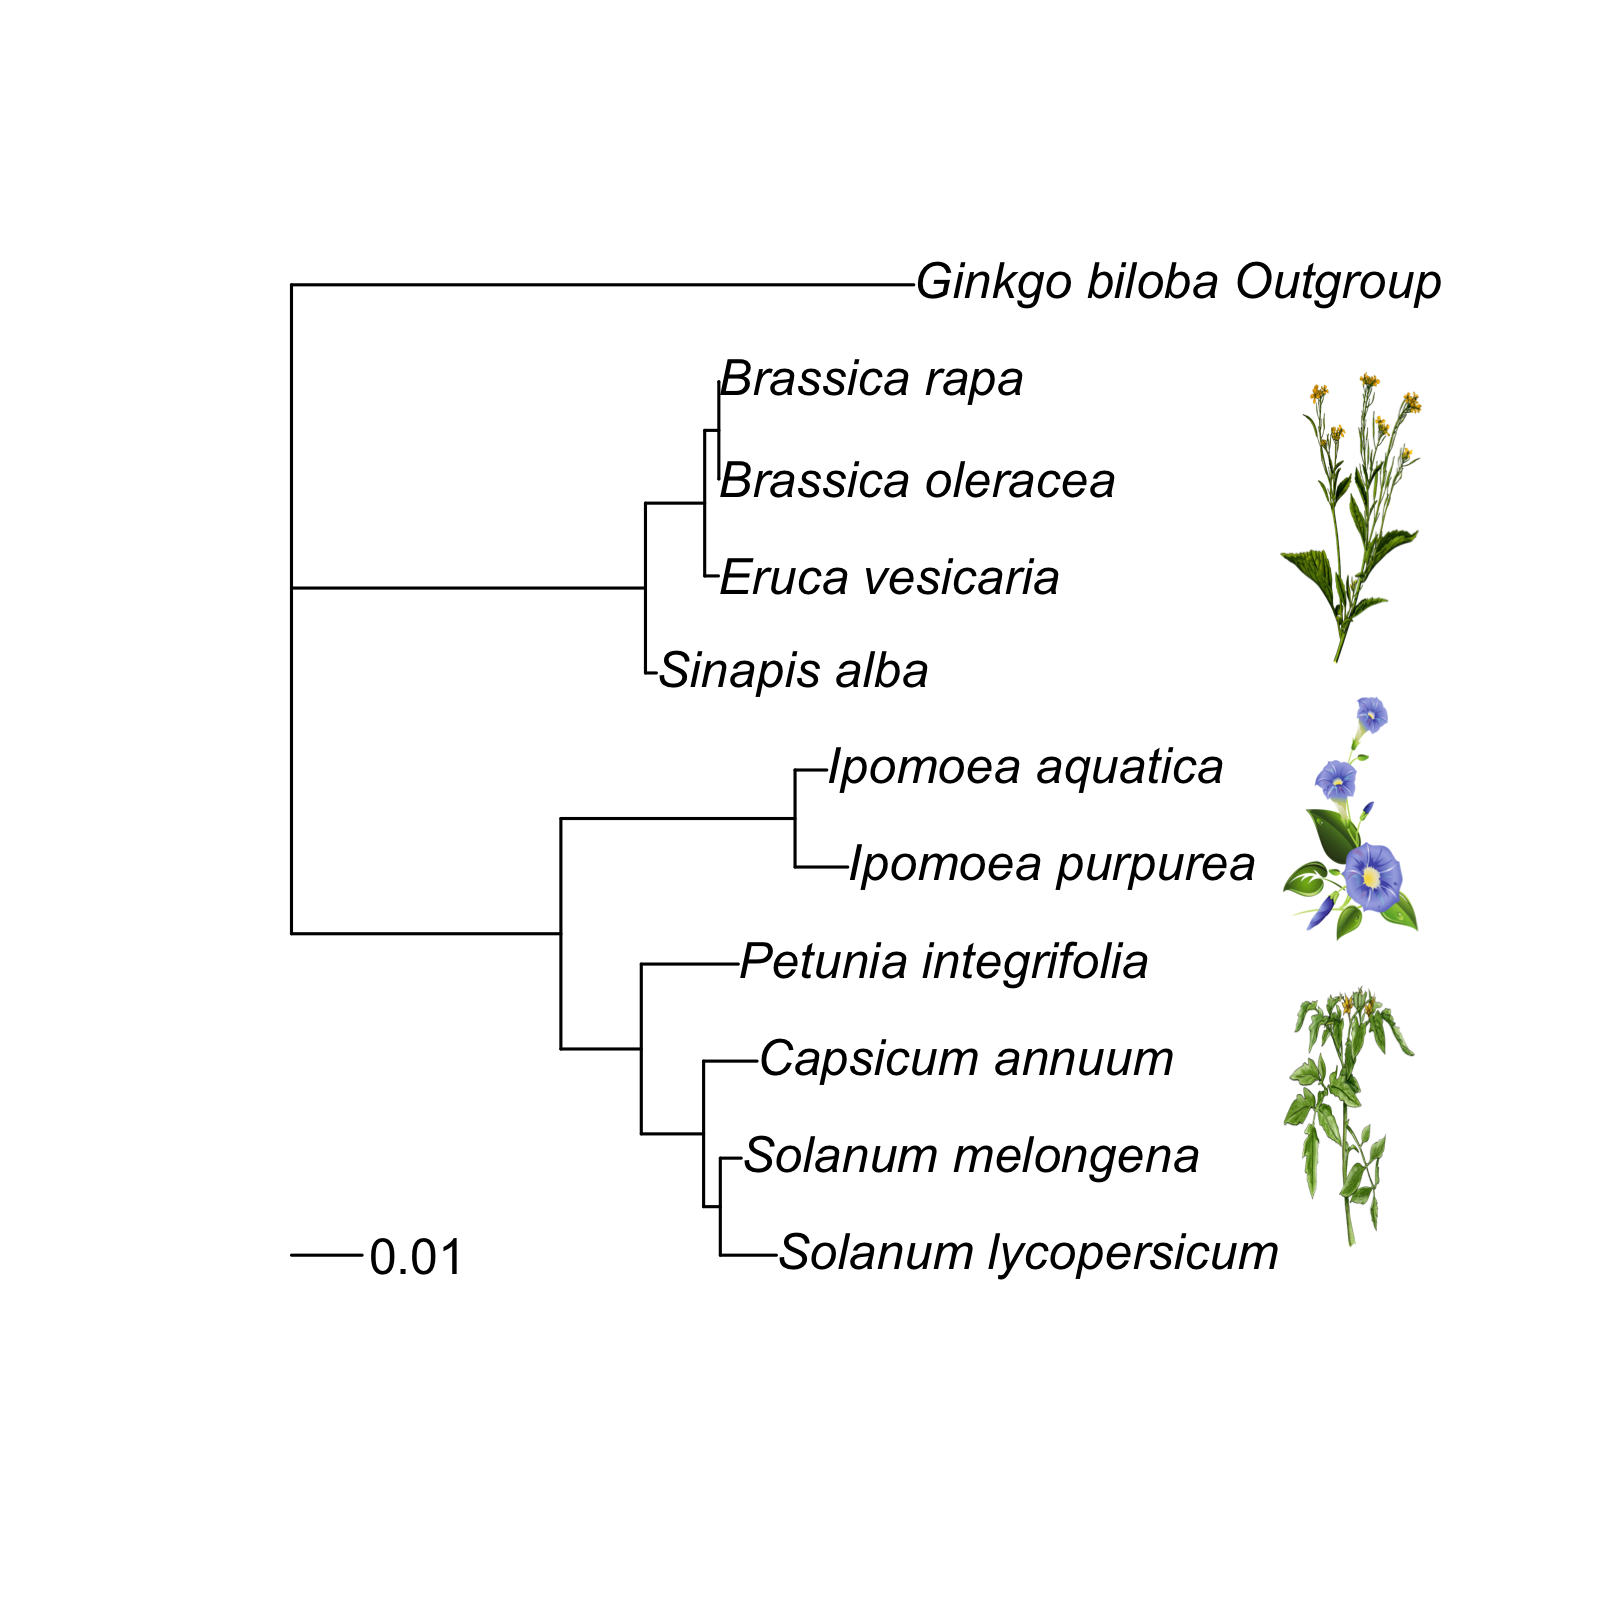
\includegraphics[width=1\linewidth]{images/phylo_image} \caption{Phylogenetic tree of the ten species used in the experiment from three different families from top to bottom: Brassicaceae, Convolvulaceae and Solanaceae}\label{fig:unnamed-chunk-1}
\end{figure}

\newpage

\textbf{Table 1} Species list with family and genus.

\begin{longtable}[]{@{}lll@{}}
\toprule
Family & Genus & Species\tabularnewline
\midrule
\endhead
Brassicaceae & Brassica & Brassica rapa\tabularnewline
Brassicaceae & Brassica & Brassica oleracea\tabularnewline
Brassicaceae & Eruca & Eruca versicaria\tabularnewline
Brassicaceae & Sinapis & Sinapis alba\tabularnewline
Convolvulaceae & Ipomoea & Ipomoea aquatica\tabularnewline
Convolvulaceae & Ipomoea & Ipomoea purpurea\tabularnewline
Solanaceae & Capsicum & Capsicum annuum\tabularnewline
Solanaceae & Petunia & Petunia integrifolia\tabularnewline
Solanaceae & Solanum & Solanum lycopersicum\tabularnewline
Solanaceae & Solanum & Solanum melongena\tabularnewline
\bottomrule
\end{longtable}

\newpage

\textbf{Hand pollination}

Foreign pollen effect was studied through two different treatments, one
with 50\% conspecific pollen and 50\% heterospecific pollen and a second
one with 100\% foreign pollen in order to see if foreign pollen can
trigger fruit production by itself or even seeds through ovule
usurpation. Therefore, we perfomed 180 different heterospecific
treatments (N=10). Seed set was the proxy of effect for all our
treatments. Moreover, hand cross-pollination (between individuals of the
same species), hand self-pollination, apomixis (bagged emasculated
flowers) and natural selfing were tested for each species (N=10). For
the treatments with foreign pollen and hand cross-pollination, flowers
were emasculated the day prior anthesis and hand pollinated next day
with a toothpick. Hand-pollination was conducted with 3-4 gentle touches
on the stigma surface. For each species 20 anthers were collected and
their pollen counted with a hemocytometer, each anther was counted 4
times and then an average of these counts was performed. Once, the
average number of pollen grains per anther was known, the proportion of
anthers per mix was calculated in order to achieve a 50-50\% mix. To
confirm that the treatments applied were the desire proportions, the
total stigmatic load of pollen was counted and the proportions
calculated between the two species of the mix. Because pollen from the
same family was difficult to distinguish, and we expected similar
properties in mixing, we counted pollen from just one randomly selected
species within each donor family different to the focal's family (N=3).

\textbf{Traits and evolutive distance}

The traits measured for each species were pollen per anther, pollen
size, number of ovules and stigma, style, ovary width and length. For
the stigma, the stigmatic area was also measured and moreover the
stigmas were divided in wet/dry type with the help of the
stereomicroscope. All the morphometrical measurements were performed
with a stereophotomicroscope with the exception of pollen size that was
carried out with a light microscope. Pollen was counted for 20 anthers
of each species with 4 replicates per sample with an hemocytometer.
Previously, anthers were squashed on a known solution with the pippete
tip and homogeneize with a vortex for 30 seconds. Ovule number was
counted with the help of a stereomicroscope and a small grid over a
petri dish from 15 randomly selected flowers. Fruits per number of
flowers treated were counted for just Solanaceae species with fleshy
fruit. For all the species we counted the number of seeds produced per
average number of ovules. Levels of self-incompatibility were estimated
by dividing the seed set of hand self-pollination by hand
cross-pollination Lloyd and Schoen (1992).

\textbf{Analysis}

To evaluate heterospecific pollen effect on seed production we performed
linear mixed models. The distinct heterospecific pollination treatments
were compared through relevelling each variable with the cross
pollination treatment which was our control for optimum seed production
for all the species. The different replicates of each treatment were
considered as random effects. Seed production was scaled for all the
species with mean 0 and standard deviation of 1 prior to the analysis.
All the analysis were conducted with the statistical language \texttt{R}
(R Core Team 2018).

To compare the magnitude of effect of heterospecific pollen across
species we conducted standarized Hedges' d {[}(mean of mixed 50\% mix -
mean of cross pollination)/pooled SD{]} with \textbf{effsize} package.
We did in three different ways: effect sizes of each donor per focal
species; effect sizes per family of the different donors per focal
species; effect sizes of all the donors grouped per focal species.

We conducted mantel test to check for correlations between
heterospecific pollen effect and phylogenetic distance. Due to
improvents in statistical power we used the square root of the
phylogenetic distance (Letten \& Cornwell 2014). Two different
phylogenetic distances were used from two kinds of markers: 1) Internal
transcribed spacer (ITS) and 2) ribulose-bisphosphate carboxylase
(RBCL). The sequences were obtained from GenBank
(\url{https://www.ncbi.nlm.nih.gov/genbank/}, accessed 20 Oct. 2018).
The sequences were aligned with clustal omega and the pairwise evolutive
distances calculated with MEGA7.

In order to test the relative effect of traits on seed production with
foreign pollen we performed Mantel test in R (\textbf{vegan} package,
Euclidean distance) between the assymetrical matrix of heterospecific
pollen effect (10 by 10 matrix) with the different distance matrices of
traits. Heterospecific pollen effect was obtained through the
subtraction of seed production by hand cross-pollination minus seed
production of the different heterospecific pollen treatments. To find a
model with the best explanatory traits we used the function
\textbf{bioenv} from R. We also conducted Mantel test between the matrix
of heterospecific pollen effect and the distance matrix from all the
traits. Moreover, we explored also the correlation between traits and
heterospecific pollen effect through generalized mixed models where the
response variable was heterospecific pollen effect and the explanatory
variable the different traits. In addition, we tested the correlation
between the total amount of pollen deposited on the stigma with
heterospecific pollinations and the stigma size through Pearson's
correlation.

\href{Jose}{Phylogenetic signal of traits?}

Total pollen deposited on stigmas was significantly correlated with the
stigmatic area, pearsons correlation=0.57 and p-value=0.008. Proportions
of pollen talk about it to 50-50 mix? Talk aboout this in methods too.

Also the plots of ratios to appendices.

NMDS to appendix?

\section{RESULTS}\label{results}

Results of hand cross-pollination, hand self-pollination, natural
selfing and apomixis are presented in \textbf{Figure 1} (see appendix 1
for table with values). Heterospecific pollen reduced seed set
significatively with the 50-50\% heterospecific pollen treatments for
65\% of the pairwise interactions p\textless{}0.05. Moreover, average
effect sizes differed across species and across families, see
\textbf{Figure 2}. Despite some variability in the effect of the
different pollen donors per species, in general terms the effect of
heterospecific pollen from the distinct nine treatments per species was
homogeneous (see \textbf{Figure 3}), just for four species out of ten,
just one donor did not overlap the confidence intervals with other
donors. Therefore, none of the donors had a clear stronger or weaker
effect across species. When the donors were groped by family not big
differences were seen, just for \emph{S. lycopersicum} the confidence
intervals of Brassicaceae and Convolvulaceae did not overlap (see
\textbf{Figure 4}). In addition, for the 100\% hetrospecific pollen
treatments we did not find almost seed production. However, for just one
species (\emph{S. alba}) the control pollination and the heterospecific
pollination with pollen from a confamilial had similar seed production.
For two Solanaceae species \emph{S. melongena} and \emph{C. annuum}
100\% pollen treatments produced few seedles fruits (3\% and 9\%
respectively) and they did not for the apomictic treatments.

Results of Mantel test between heterospecific pollen effect and
phylogenetic distance gave a positive statistically clear correlation
for both markers (p\textless{}0.05). The correlations with ITS and RBCL
markers was respectively of 0.29 and 0.25. We found a significant
phylogenetic signal of traits for pollen size, stigma measurements and
style length (p\textless{}0.05). Although with a lack of a significant
correlation pagel's lambda values were also relatively high
(\textgreater{}0.45) for incompatibility index, ovary length and levels
of selfing. Moreover, Mantel test between heterospecific pollen effect
and traits gave also a positive significant correlation with a r value
of 0.4. When the effect was look trait by trait with Mantel test, stigma
type and stigma measurements (length, width and area) gave a significant
positive correlation with heterospecific pollen effect.

\href{Jose}{explain ratios and total pollen} \href{}{add table with
morphometrical traits to appendix}

\newpage

\begin{figure}

{\centering 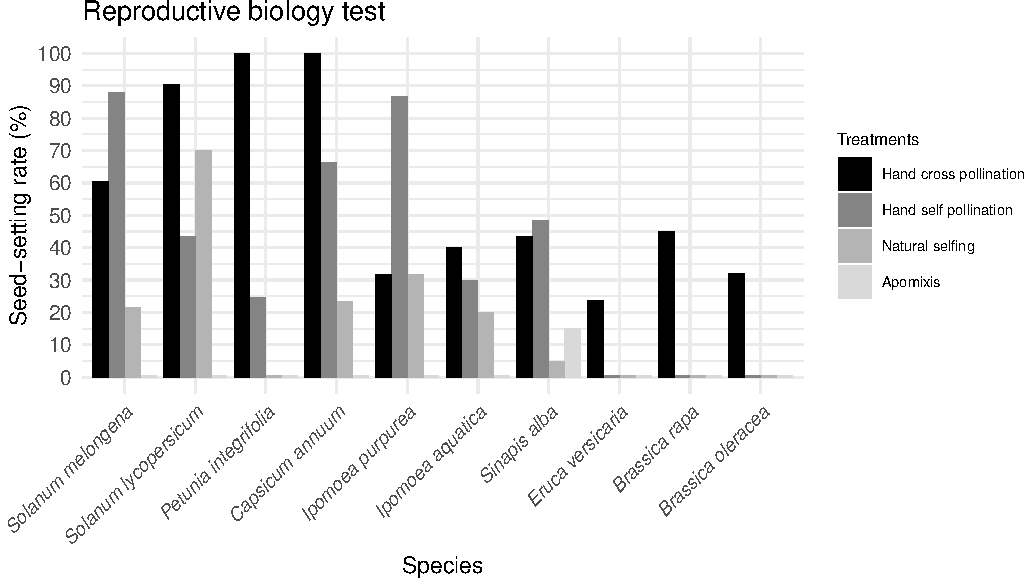
\includegraphics{output/figures/unnamed-chunk-3-1} 

}

\caption{Barplot with the different treatments that provide information of the reproductive biology of the ten species. The y axis is the proportion of ovules converted to seed in percentage. The different treatments (N=10) which are presented in the legend are, hand cross-pollination, hand self-pollination, natural selfing and apomixis. More information about these treatments can be found in Methods and Appendices.}\label{fig:unnamed-chunk-3}
\end{figure}

\newpage

\begin{figure}
\centering
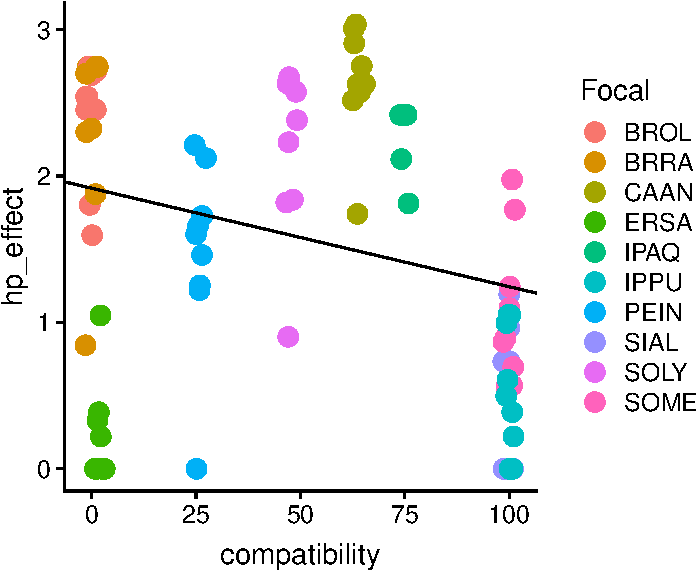
\includegraphics{output/figures/unnamed-chunk-4-1.pdf}
\caption{Average effect size and confidence intervals (95\%) of the 9
heterospecific treatments of 50\% pollen to the different 10 focal
species coloured by family.}
\end{figure}

\newpage

\begin{figure}
\centering
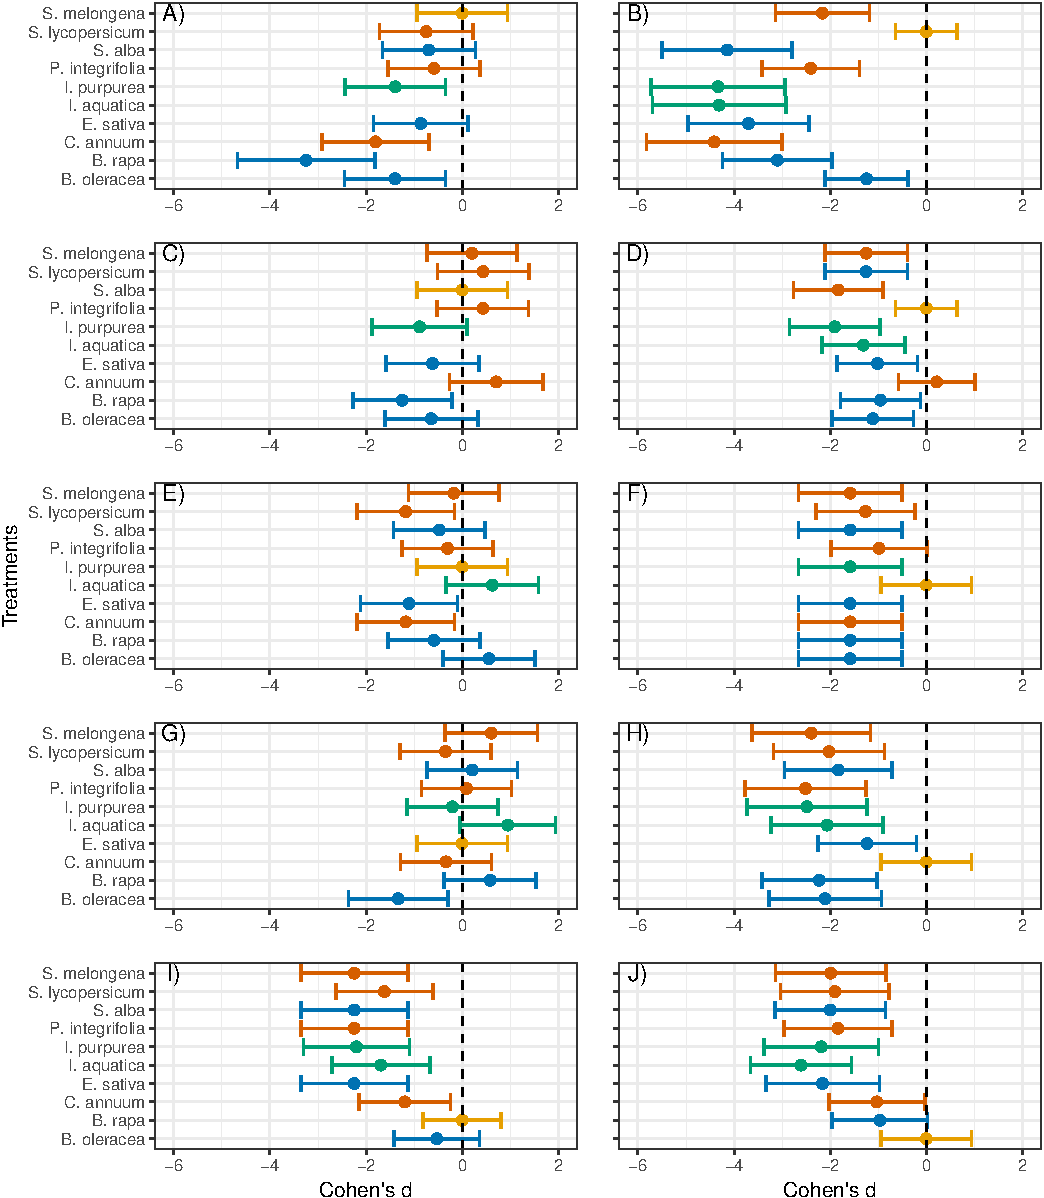
\includegraphics{output/figures/unnamed-chunk-5-1.pdf}
\caption{Effect sizes for the 10 different species. The different
families appear with different colours, when a species was focal was
coloured differently from its family.}
\end{figure}

\begin{verbatim}
TableGrob (5 x 5) "guide-box": 2 grobs
                                    z     cells                  name
99_71de3e2d00a18a2081dc4ff65135fb9d 1 (3-3,3-3)                guides
                                    0 (2-4,2-4) legend.box.background
                                              grob
99_71de3e2d00a18a2081dc4ff65135fb9d gtable[layout]
                                    zeroGrob[NULL]
\end{verbatim}

\newpage

\begin{figure}
\centering
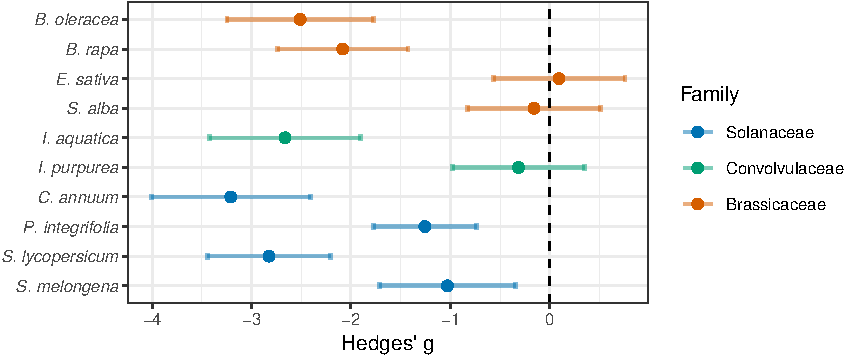
\includegraphics{output/figures/unnamed-chunk-6-1.pdf}
\caption{A}
\end{figure}

\newpage

\begin{figure}
\centering
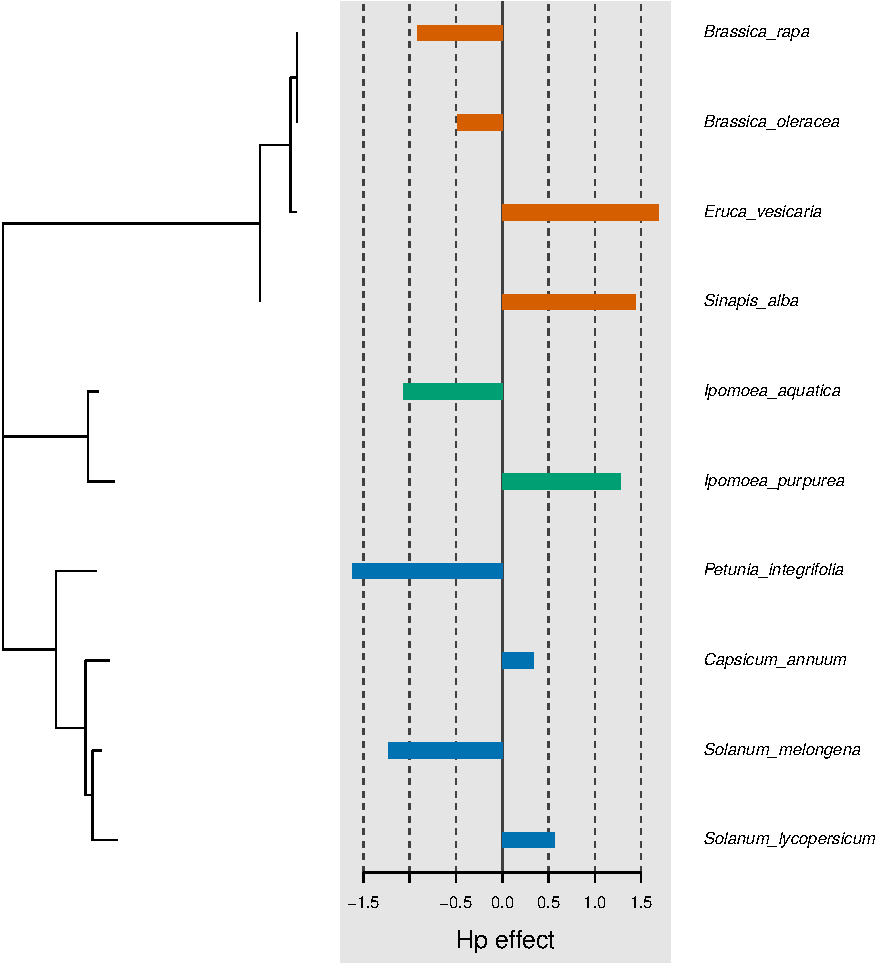
\includegraphics{output/figures/unnamed-chunk-7-1.pdf}
\caption{Phylogenetic signal of the average heterospecific pollen effect
size per species}
\end{figure}

\newpage

\section{DISCUSSION}\label{discussion}

Interestingly the effect of the different donors per species were very
homogeneous which lead us to think that the female reproductive traits
of the pollen recipient are the main ones in explaining heterospecific
pollen effect. Our main predictive trait of effect is stigma size, and
because we found a correlation between the pollen quantity deposited on
the stigma and stigma size, we argue that that the total load of pollen
deposited per treatment can obscured what are the main traits in driving
heterospecific pollen effect.

Curiously between the species with greater effect sizes, we found
completely self incompatible species, species with the smallest stigma
and the species with shortes style. Develop more\ldots{}

Although we have found a positive correlation between phylogenetic
distance and heterospecific pollen effect, this results have to be
treated carefully. From our results we want to highlight that also far
related species can affect negatively fitness but the effect from close
related is species can also have important detrimental effects.
Moreover, the effect of close related species can be masked by the
possibility of hibridization as it occure between two of our species of
Brassica. Moreover, although different effect between distinct donors
can occur we want to note the importance on the traits of the recipient
that determine an homogeneous effect between donors as we have shown in
figure xxx. These different traits will define how it will be the effect
across the different species independently of the nature of the donor
and also differently even between species of . Although traditionally
the nature of the pollen donor have been very studied, the
recipient\ldots{}

Herbs vs tress, annual vs perennial\ldots{} Many flowers vs few flowered
species; structural composition on a system

What are the implications of the findings?

\section{CONCLUSIONS}\label{conclusions}

\section{ACKNOWLEDGEMENTS}\label{acknowledgements}

\section{REFERENCES}\label{references}

\hypertarget{refs}{}
\hypertarget{ref-aizen2007}{}
Aizen, M. A., and L. D. Harder. 2007. Expanding the limits of the
pollen-limitation concept: Effects of pollen quantity and quality.
Ecology 88:271--281.

\hypertarget{ref-arceo2011}{}
Arceo-Gómez, G., and T.-L. Ashman. 2011. Heterospecific pollen
deposition: Does diversity alter the consequences? New Phytologist
192:738--746.

\hypertarget{ref-arceo2016}{}
Arceo-Gómez, G., and T.-L. Ashman. 2016. Invasion status and
phylogenetic relatedness predict cost of heterospecific pollen receipt:
Implications for native biodiversity decline. Journal of Ecology
104:1003--1008.

\hypertarget{ref-ashman2013}{}
Ashman, T.-L., and G. Arceo-Gómez. 2013. Toward a predictive
understanding of the fitness costs of heterospecific pollen receipt and
its importance in co-flowering communities. American Journal of Botany
100:1061--1070.

\hypertarget{ref-bartomeus2008}{}
Bartomeus, I., J. Bosch, and M. Vilà. 2008. High invasive pollen
transfer, yet low deposition on native stigmas in a carpobrotus-invaded
community. Annals of Botany 102:417--424.

\hypertarget{ref-carvalheiro2014}{}
Carvalheiro, L. G., J. C. Biesmeijer, G. Benadi, J. Fründ, M. Stang, I.
Bartomeus, C. N. Kaiser-Bunbury, M. Baude, S. I. Gomes, V. Merckx, and
others. 2014. The potential for indirect effects between co-flowering
plants via shared pollinators depends on resource abundance,
accessibility and relatedness. Ecology letters 17:1389--1399.

\hypertarget{ref-engel2003}{}
Engel, E. C., and R. E. Irwin. 2003. Linking pollinator visitation rate
and pollen receipt. American Journal of Botany 90:1612--1618.

\hypertarget{ref-fang2013}{}
Fang, Q., and S.-Q. Huang. 2013. A directed network analysis of
heterospecific pollen transfer in a biodiverse community. Ecology
94:1176--1185.

\hypertarget{ref-galen1989}{}
Galen, C., and T. Gregory. 1989. Interspecific pollen transfer as a
mechanism of competition: Consequences of foreign pollen contamination
for seed set in the alpine wildflower, polemonium viscosum. Oecologia
81:120--123.

\hypertarget{ref-inouye1980}{}
Inouye, D. W. 1980. The terminology of floral larceny. Ecology
61:1251--1253.

\hypertarget{ref-letten2015}{}
Letten, A. D., and W. K. Cornwell. 2015. Trees, branches and (square)
roots: Why evolutionary relatedness is not linearly related to
functional distance. Methods in Ecology and Evolution 6:439--444.

\hypertarget{ref-lloyd1992}{}
Lloyd, D. G., and D. J. Schoen. 1992. Self-and cross-fertilization in
plants. i. functional dimensions. International Journal of Plant
Sciences 153:358--369.

\hypertarget{ref-magrach2017}{}
Magrach, A., J. P. González-Varo, M. Boiffier, M. Vilà, and I.
Bartomeus. 2017. Honeybee spillover reshuffles pollinator diets and
affects plant reproductive success. Nature ecology \& evolution 1:1299.

\hypertarget{ref-montgomery2012}{}
Montgomery, B. R., and B. J. Rathcke. 2012. Effects of floral
restrictiveness and stigma size on heterospecific pollen receipt in a
prairie community. Oecologia 168:449--458.

\hypertarget{ref-morales2008}{}
Morales, C. L., and A. Traveset. 2008. Interspecific pollen transfer:
Magnitude, prevalence and consequences for plant fitness. Critical
Reviews in Plant Sciences 27:221--238.

\hypertarget{ref-murphy1995}{}
Murphy, S. D., and L. W. Aarssen. 1995. Reduced seed set in elytrigia
repens caused by allelopathic pollen from phleum pratense. Canadian
Journal of Botany 73:1417--1422.

\hypertarget{ref-neiland1999}{}
Neiland, M., and C. Wilcock. 1999. The presence of heterospecific pollen
on stigmas of nectariferous and nectarless orchids and its consequences
for their reproductive success. Protoplasma 208:65--75.

\hypertarget{ref-pauw2013}{}
Pauw, A. 2013. Can pollination niches facilitate plant coexistence?
Trends in ecology \& evolution 28:30--37.

\hypertarget{ref-R_Core_Team_2018}{}
R Core Team. 2018. R: A language and environment for statistical
computing. R Foundation for Statistical Computing, Vienna, Austria.

\hypertarget{ref-thomson1982}{}
Thomson, J. D., B. J. Andrews, and R. Plowright. 1982. The effect of a
foreign pollen on ovule development in diervilla lonicera
(caprifoliaceae). New Phytologist 90:777--783.

\hypertarget{ref-tong2016}{}
Tong, Z.-Y., and S.-Q. Huang. 2016. Pre-and post-pollination interaction
between six co-flowering pedicularis species via heterospecific pollen
transfer. New Phytologist 211:1452--1461.

\hypertarget{ref-waser1996}{}
Waser, N. M., L. Chittka, M. V. Price, N. M. Williams, and J. Ollerton.
1996. Generalization in pollination systems, and why it matters. Ecology
77:1043--1060.

\hypertarget{ref-whitehead2018}{}
Whitehead, M. R., R. Lanfear, R. J. Mitchell, and J. D. Karron. 2018.
Plant mating systems often vary widely among populations. Frontiers in
Ecology and Evolution 6:38.

\hypertarget{ref-williams1990}{}
Williams, E., and J. Rouse. 1990. Relationships of pollen size, pistil
length and pollen tube growth rates in rhododendron and their influence
on hybridization. Sexual Plant Reproduction 3:7--17.

\section{APPENDIX}\label{appendix}

\begin{enumerate}
\def\labelenumi{\arabic{enumi}.}
\item
\end{enumerate}

\textbf{Table S1}. Perecentage of seeds produced per ovule for the ten
species used in the experiment. The treatments presented are hand
cross-pollination, hand self-pollination, natural selfing and apomixis
(emasculated flowers).

\begin{longtable}[]{@{}lrrrr@{}}
\toprule
Species & Cross & Self & Natural\_selfing & Apomixis\tabularnewline
\midrule
\endhead
Brassica oleracea & 32.06897 & 0.0000000 & 0.00000 & 0\tabularnewline
Brassica rapa & 44.97041 & 0.0000000 & 0.00000 & 0\tabularnewline
Eruca versicaria & 23.75000 & 0.4166667 & 0.00000 & 0\tabularnewline
Sinapis alba & 43.33333 & 48.3333333 & 5.00000 & 15\tabularnewline
Ipomoea aquatica & 40.00000 & 30.0000000 & 20.00000 & 0\tabularnewline
Ipomoea purpurea & 31.66667 & 86.6666667 & 31.66667 & 0\tabularnewline
Capsicum annuum & 100.00000 & 66.2240664 & 23.48548 & 0\tabularnewline
Petunia integrifolia & 100.00000 & 24.7727273 & 0.00000 &
0\tabularnewline
Solanum lycopersicum & 90.38043 & 43.4782609 & 70.00000 &
0\tabularnewline
Solanum melongena & 60.47525 & 87.9702970 & 21.56436 & 0\tabularnewline
\bottomrule
\end{longtable}

\begin{enumerate}
\def\labelenumi{\arabic{enumi}.}
\setcounter{enumi}{1}
\item
\end{enumerate}

\textbf{Figure S1}. Pollen ratios separated by family A) Brassicaceae,
B) Solanaceae, C) Convolvulaceae. Pollen was counted for crosses with
species of the other two families (N=3). To prepare these ratios all the
pollen grains on the stigma were counted.

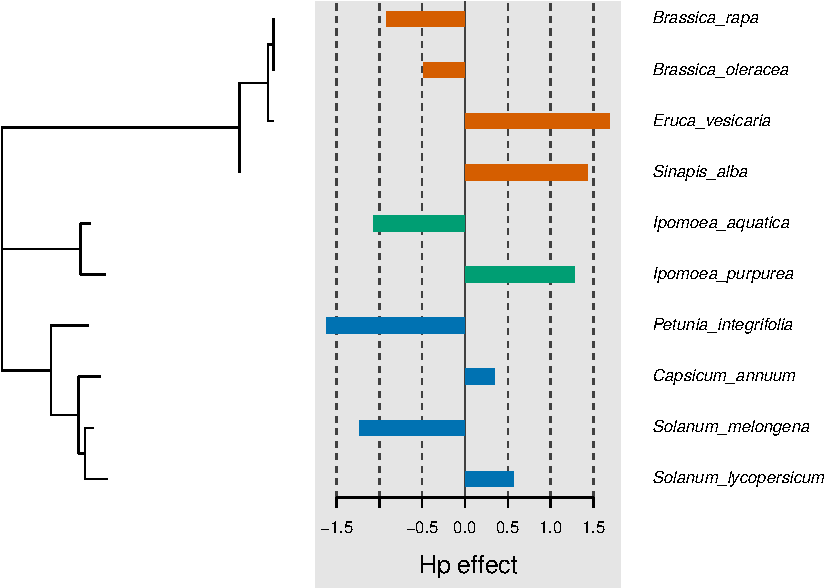
\includegraphics{output/figures/unnamed-chunk-9-1.pdf}
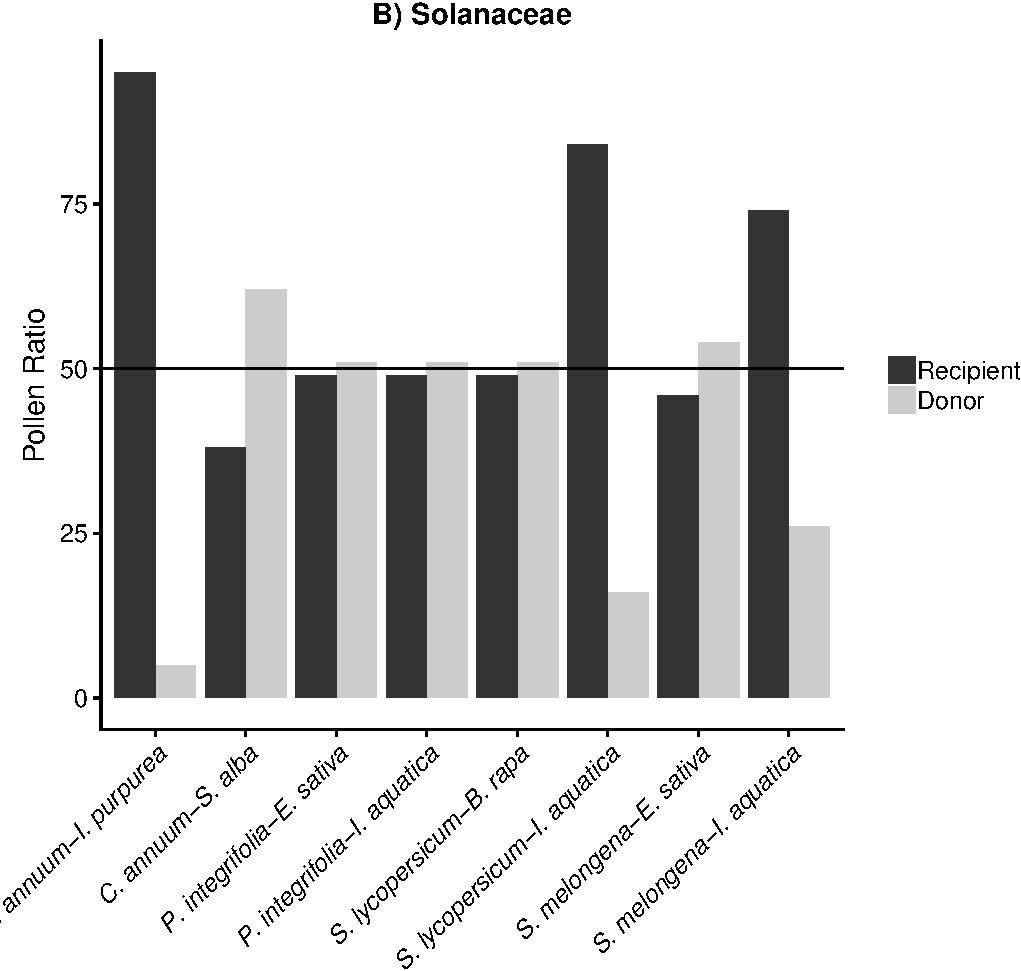
\includegraphics{output/figures/unnamed-chunk-9-2.pdf}
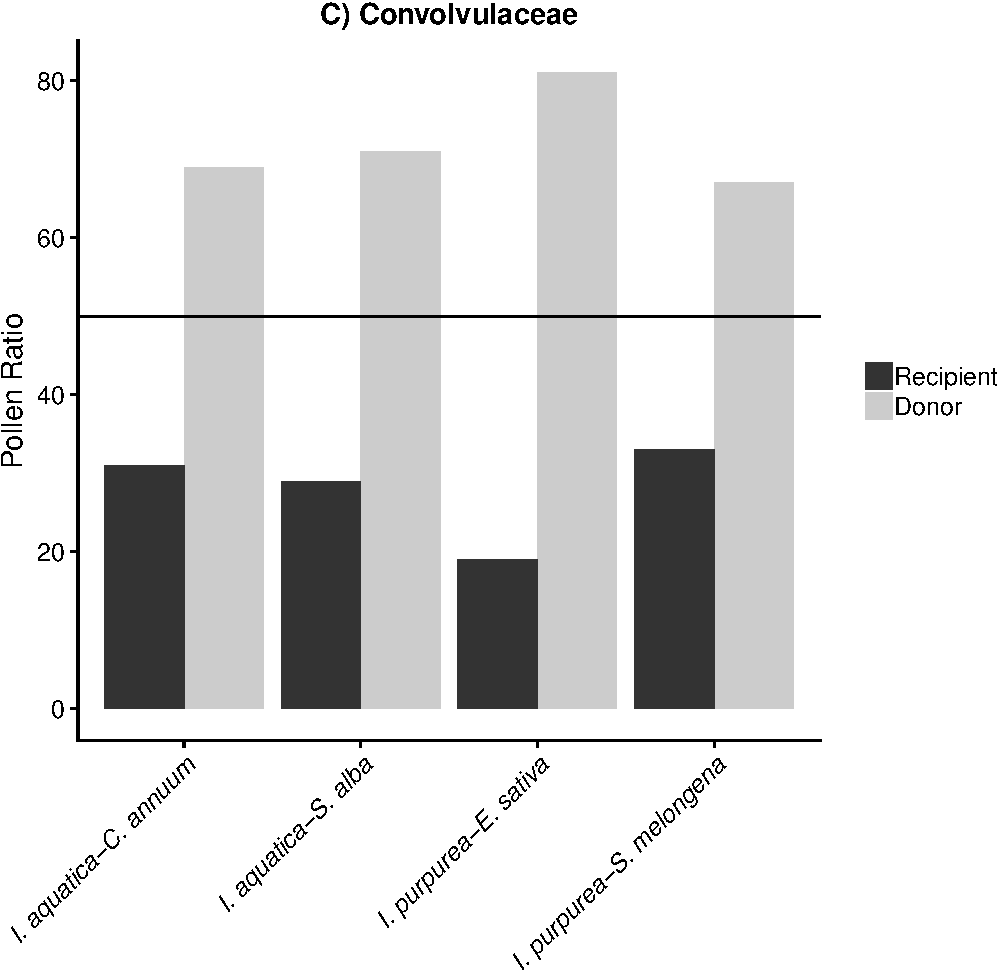
\includegraphics{output/figures/unnamed-chunk-9-3.pdf}

\eleft

\clearpage

\listoftables

\newpage

\newpage

\clearpage

\listoffigures

\newpage

\newpage

\blandscape

\elandscape

\clearpage

\end{document}